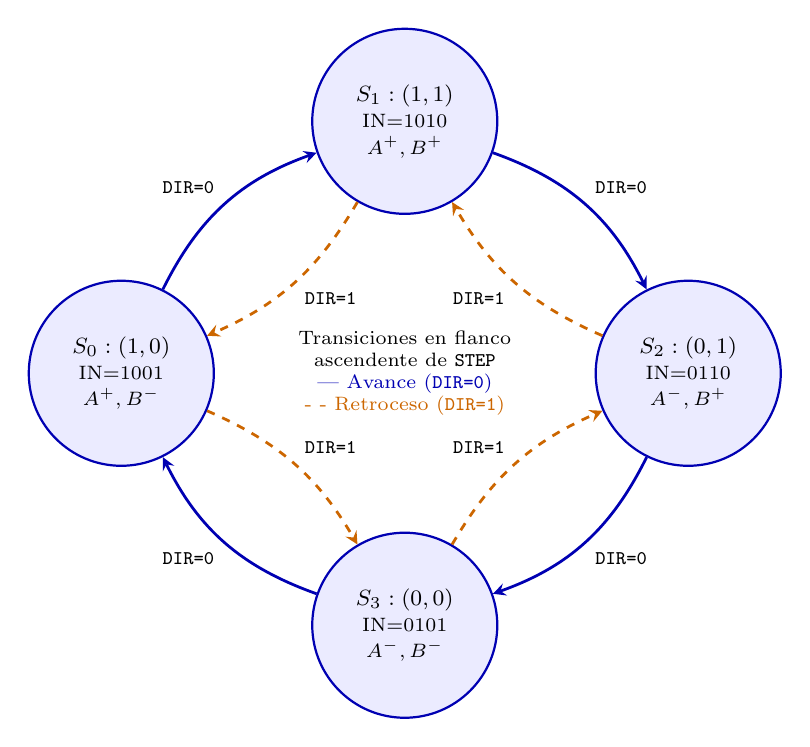
\begin{tikzpicture}[
  >=stealth, thick,
  state/.style={
    draw=blue!70!black, fill=blue!8, circle, minimum size=2.35cm, align=center, font=\footnotesize
  },
  fwd/.style={->, draw=blue!70!black, line width=1pt},
  rev/.style={->, draw=orange!80!black, line width=1pt, dashed}
]

  \node[state] (s0) at (-3.6,0) {\textbf{$S_0: (1,0)$}\\{\scriptsize IN=1001}\\{\scriptsize $A^+, B^-$}};
  \node[state] (s1) at (0,3.2)  {\textbf{$S_1: (1,1)$}\\{\scriptsize IN=1010}\\{\scriptsize $A^+, B^+$}};
  \node[state] (s2) at (3.6,0)  {\textbf{$S_2: (0,1)$}\\{\scriptsize IN=0110}\\{\scriptsize $A^-, B^+$}};
  \node[state] (s3) at (0,-3.2) {\textbf{$S_3: (0,0)$}\\{\scriptsize IN=0101}\\{\scriptsize $A^-, B^-$}};

  % Avance DIR = 0 (sentido horario)
  \draw[fwd] (s0) to[bend left=22] node[above left, font=\scriptsize] {\texttt{DIR=0}} (s1);
  \draw[fwd] (s1) to[bend left=22] node[above right, font=\scriptsize] {\texttt{DIR=0}} (s2);
  \draw[fwd] (s2) to[bend left=22] node[below right, font=\scriptsize] {\texttt{DIR=0}} (s3);
  \draw[fwd] (s3) to[bend left=22] node[below left, font=\scriptsize] {\texttt{DIR=0}} (s0);

  % Retroceso DIR = 1 (sentido antihorario)
  \draw[rev] (s1) to[bend left=18] node[below right, font=\scriptsize] {\texttt{DIR=1}} (s0);
  \draw[rev] (s2) to[bend left=18] node[below left, font=\scriptsize] {\texttt{DIR=1}} (s1);
  \draw[rev] (s3) to[bend left=18] node[above left, font=\scriptsize] {\texttt{DIR=1}} (s2);
  \draw[rev] (s0) to[bend left=18] node[above right, font=\scriptsize] {\texttt{DIR=1}} (s3);

  % Leyenda central
  \node[align=center, font=\scriptsize] at (0,0) {
    Transiciones en flanco\\ascendente de \texttt{STEP}\\
    {\color{blue!70!black}--- Avance (\texttt{DIR=0})}\\
    {\color{orange!80!black}- - Retroceso (\texttt{DIR=1})}
  };
\end{tikzpicture}
